\documentclass[conference]{IEEEtran}
\usepackage[utf8]{inputenc}
\usepackage{cite}
\usepackage{amsmath,amssymb,amsfonts}
\usepackage{algorithmic}
\usepackage{graphicx}
\usepackage{textcomp}
\usepackage{xcolor}
\usepackage{blindtext}
\usepackage{hyperref}
\def\BibTeX{{\rm B\kern-.05em{\sc i\kern-.025em b}\kern-.08em
		T\kern-.1667em\lower.7ex\hbox{E}\kern-.125emX}}

\begin{document}
	
	\title{Simulating the green-beard effect with selective altruism}
	
	\author{\IEEEauthorblockN{L. Yeh}
		\IEEEauthorblockA{\textit{Faculty of Science, Utrecht University, Utrecht, The Netherlands}\\
		(Dated: \today)} 
	}
	
	\maketitle
	
	\begin{abstract}
	The green-beard effect can be simulated by having two groups of individuals. One of the groups are regular individuals, and another are individuals with a green-beard gene. An analysis of the simulations results shows that individuals with a green-beard gene are more likely to survive than individuals without the gene. Even if the starting population size of the green-beard is significantly lower than the starting population size of the regular.
	\end{abstract}
	
	\section{Introduction}
	The green-beard effect is a hypothetical theory used in evolutionary biology to explain how altruism works among individuals \cite{hamilton1964genetical}. It is an idea coined by W.D. Hamilton, a British evolutionary biologist. Hamilton claims that altruistic behaviour can favour a species containing that trait. The name of 'green-beard' stems from 'The selfish gene', a book written by R. Dawkins \cite{dawkins2017selfish}. In biology, altruism's definition refers to the action of certain individuals that aims to increase the fitness of another individual, at the cost of their own fitness \cite{barrett2008natural}. 
	
	A green-beard is an individual that has a certain 'green-beard' gene that can make other green-beards recognize each other. Green-beards are altruistic individuals, meaning that they will aim to help each other even if the action will make them lose fitness \cite{gardner2010greenbeards}. Hamilton argues that bearers of the green-beard gene are favoured by natural selection. This implies that the reproductive family members of the green-beard gene have a better chance of survival than those who do not.
	
	\section{Methods}
	The experiment aims to discover the effect of selective altruism by using individuals with and without a green-beard gene. This is done by simulating a world consisting of two species. One with the green-beard gene, called green-beards. The other without the green-beard gene, called regulars. These species will each have to find food. If they are able to find food, they will survive one generation and thus, reproduce offspring. Those who do not find food will die and will not be able to reproduce. Due to the altruistic behaviour of green-beards, the green-beards are able to share their food with other green-beards. If the green-beard has found extra food, the green-beard can share it's food with another. 
	
	Every individual has the same chance of finding food. The amount of food is equal to the population size. However, only green-beards are able to share their food.
	
	In this experiment, the species that ends up with a higher population size  will be considered the one with the better strategy. The species with a higher population size $p$ will be the one who is able to adapt the best to the world, which is the definition of natural selection \cite{fisher1958genetical}.
	
	\section{Results}
	Running the simulation can give us various results depending on the parameters. The amount of simulations have been run for $S = 500$, and generations $G = 150$. The model has run with a population size of 1000 regulars $p_r$ and 1000 green-beards $p_g$. The figures showcase the average population size over the amount of simulations $L$. Figure \ref{fig:50-50} shows that the more generations that follow, the $p_g$ increases, whilst the population $p_r$ decreases. This implies that the green-beards are better at survival than regulars. 

	\begin{figure}[htbp]
		\centerline{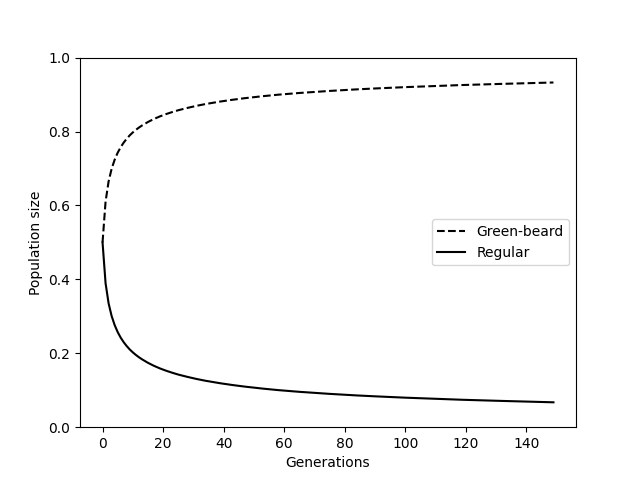
\includegraphics[scale=0.5]{figures/50-50.png}}
		\caption{Results of a simulation where the population of green-beards and regulars start off the same.}
		\label{fig:50-50}
	\end{figure}
	
	Running the simulation with $L = 500$ and $G = 150$ on a simulation with starting populations $p_r = 1000$ and $p_g = 500$, the result shows that even with a smaller starting population size, the green-beards will eventually take over the regulars in terms of population size, as shown in Figure \ref{fig:1000-500}.

	\begin{figure}[htbp]
		\centerline{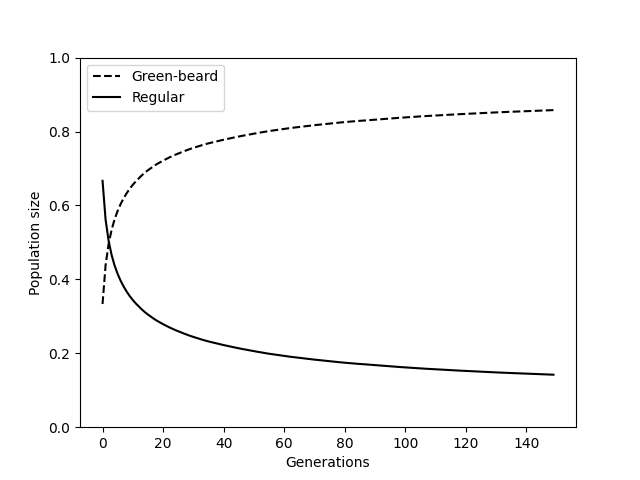
\includegraphics[scale=0.5]{figures/1000-500.png}}
		\caption{Results of a simulation where the starting population $p_g = 500$ of green-beards are significantly lower than the starting population $p_r = 1000$ of regulars.}
		\label{fig:1000-500}
	\end{figure}

	\section{Conclusion and Discussion}
	The results from the simulations show that individuals with the green-beard gene are better at survival than individuals who don't share that gene. In the simulation, even if the starting population of the green-beards is smaller than the starting population of the regulars, the green-beards will eventually exceed the population of regulars. This concludes that the green-beards are better at survival than regulars.
	
	Although currently only the green-beards and regulars are compared with each other, Hamilton's theory also include other individuals \cite{hamilton1964genetical}. An example of an individual is a green-beard that has the green-beard gene, but does not have altruism. This individual can get help from green-beards, whilst not providing any help. In future experiments, this type of individual can also be included in the comparison.
	
\bibliographystyle{plain}
\bibliography{references.bib}
	
\end{document}
